\documentclass{szzclass}
\usepackage[czech]{babel}
\usepackage[margin=3cm]{geometry}
\usepackage{hyperref}

% \subject{SAP}
% \code{BI-SPOL-27}
% \topic{Kombinační a sekvenční logické obvody (Mealy, Moore), popis a možnosti implementace na úrovni hradel. Minimalizace vyjádření logické funkce (s využitím map).}

\begin{document}
\section{Kombinační a sekvenční logické obvody (Mealy, Moore)}
\subsection{Kombinační}
Výstup je dán kombinací vstupů, nezáleží na stavu. \\
Matematický model -- logická funkce.
\subsection{Sekvenční}
Výstup závisí na posloupnosti vstupů, realizuje se zpětnými vazbami. \\
Matematický model -- konečný automat.
\begin{description}
\item[asynchronní] bez hodinového vstupu
\item[synchronní] s hodinovým vstupem
\end{description}

\subsection{Moore}
Reaguje na vstup až při přechodu do dalšího stavu. Výstup je v uzlech.

\subsection{Mealy}
Reaguje na vstup ihned. Výstup je v přechodech.

\section{Popis a možnosti implementace na úrovni hradel.}
Kombinační obvody lze popsat:
\begin{itemize}
  \item Logická funkce (např.: $X = \overline{A}\cdot B + A\cdot B$)
  \item Mapa
  \item Krychle
  \item Tabulka
  \item Graf přechodů
  \item Popis stavů a přechodových funkcí (např.: $(X,Y,S,S_0,\delta,\lambda)$)
\end{itemize}

\begin{tabular}{l l}
$X$ & \dots množina vstupních symbolů \\
$Y$ & \dots množina výstupních symbolů \\
$S$ & \dots množina stavů \\
$S_0$ & \dots počáteční stav \\
$\delta(s\in S)$ & \dots výstupní funkce u Moorea\\
$\delta(s\in S,x\in X)$ & \dots výstupní funkce u Mealyho\\
$\lambda(s\in S,x\in X)$ & \dots přechodová funkce
\end{tabular}

\subsection{Na úrovni hradel - diagram}
(N)AND, (N)OR, (N)XOR, NOT

\begin{figure}[h]
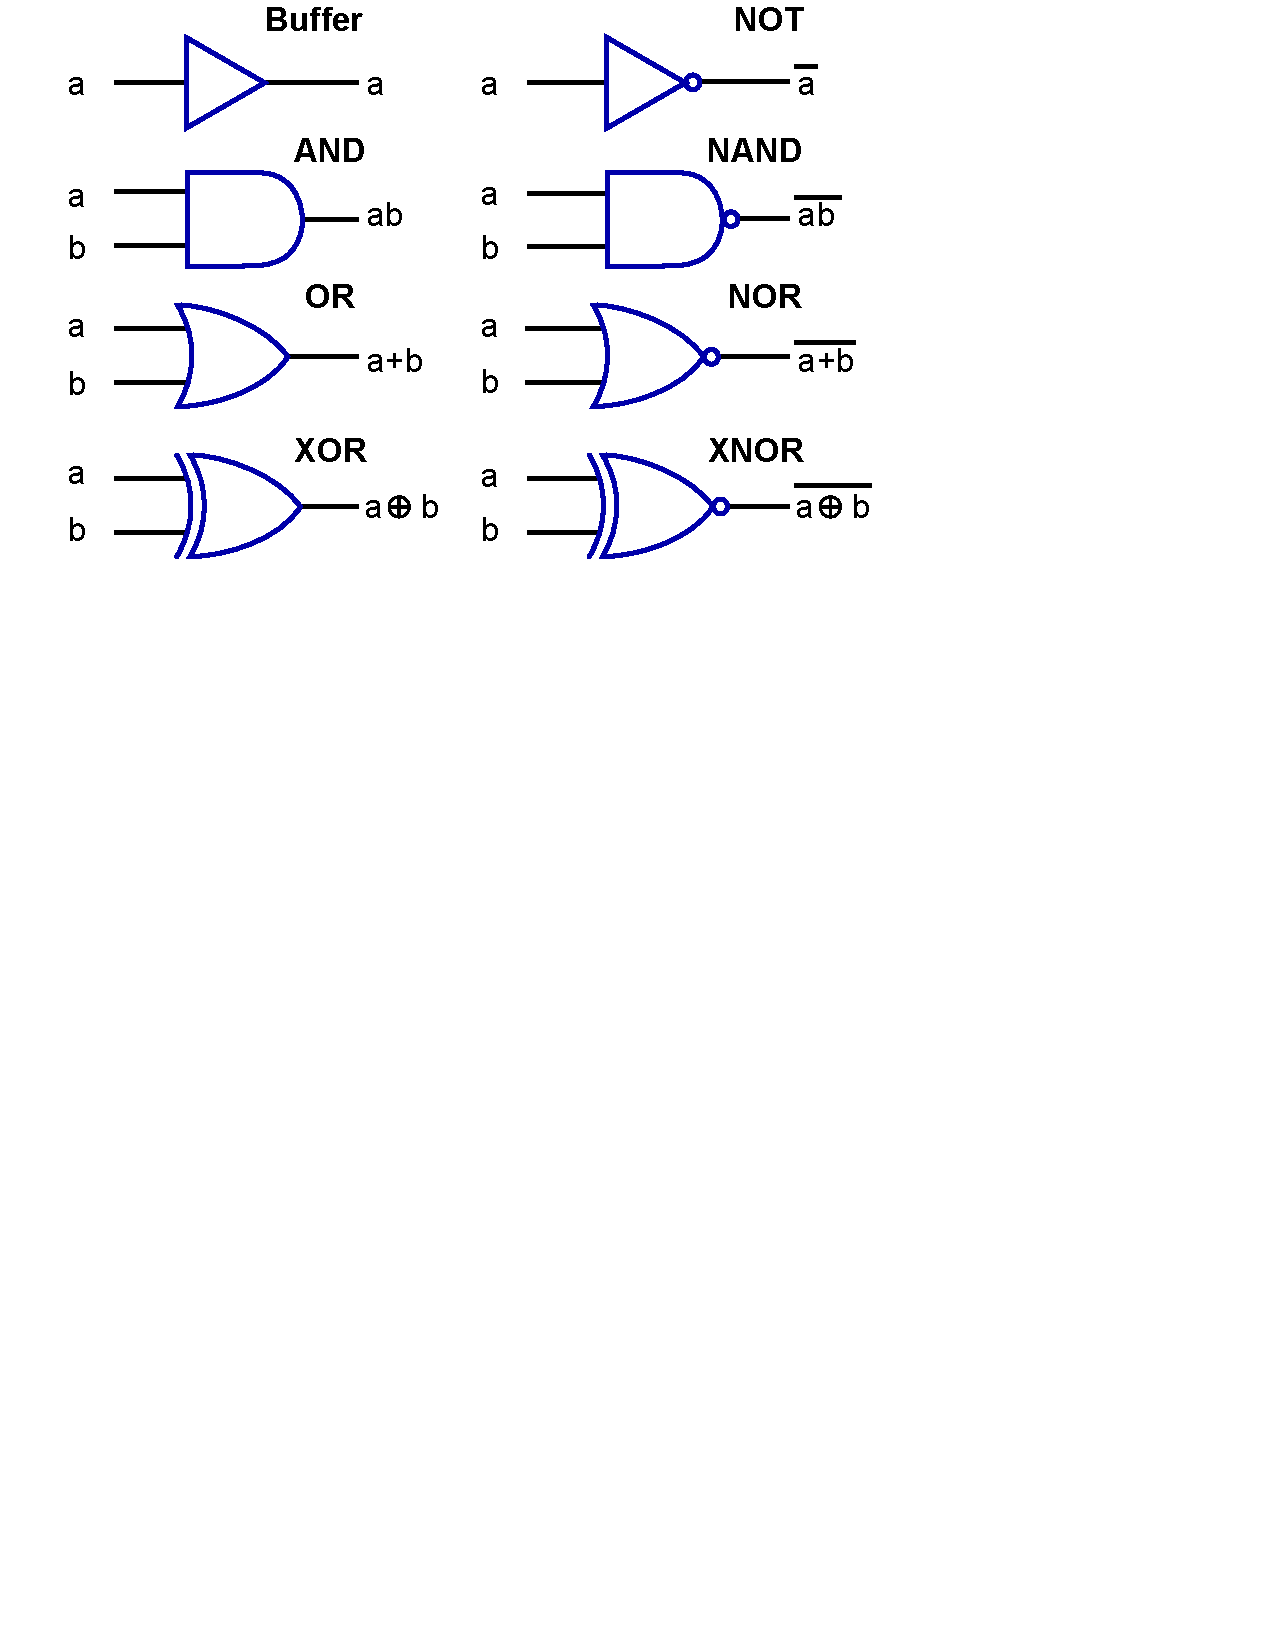
\includegraphics[width=8cm]{gates}
\end{figure}

\begin{description}
  \item [Dekodér 1 z N] -- vybírám adresu, aby mi svítila jedna žárovka
  \item [Multiplexor] -- vybírám bit, kterej chci \uv{poslat}, přes jeden kabel
  \item [Demultiplexor] -- opak multiplexoru
  \item [Sčítačka (poloviční, úplná)] -- sčítá dva bity (ta úplná počítá i s přenosem z předchozích řádů). Úplné sčítačky se dají nakombinovat, aby se dalo sečíst binární číslo.
\end{description}

\section{Minimalizace vyjádření logické funkce (s využitím map).}
\begin{itemize}
  \item MNDF - minimální normální disjunktní forma
  \item MNKF - minimální normální konjunktivní forma
\end{itemize}

\subsection{Postup pro vytvoření MNDF}
\begin{enumerate}
  \item Napíšu si pravdivostní tabulku, co chci za vstupy.
  \item Zapíšu jedničky (případně křížky - Don't care) do Karnaugovy mapy.
  \item V mapě najdu co největší skupiny o velikostech mocnin.
  \item Skupiny přepíšu do funkce tak, že zapíšu proměnné, které nemění svoji hodnotu.
\end{enumerate}

\begin{figure}[h]
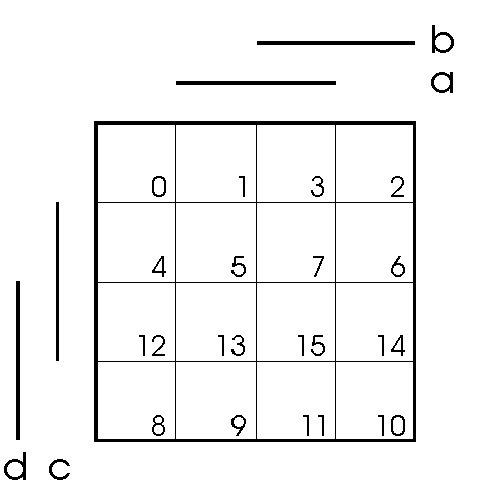
\includegraphics[width=8cm]{karnaugh}
\end{figure}

Příklady na procvičení jsou na \url{https://courses.fit.cvut.cz/BI-SAP/media/seminars/kap3.pdf}.
\end{document}
